\title{Controller für Remotekamerasystem}

\team{%
    Marius Hasler,
    Christian Häni}

\client{BBM Productions AG}

\coaches{%
    Matthias Meier}

\fssummary{
In einem bestehenden System zur Fernsteuerung von Kameras das bei der Produktion von Fernsehinhalten bei Liveübertragung zum Einsatz kommt, soll der zentrale Steuerkontroller mit neuer leistungsfähigerer Hardware entwickelt werden.
}

\fsgraphics{
    \begin{minipage}[t][][t]{0.5\textwidth}
        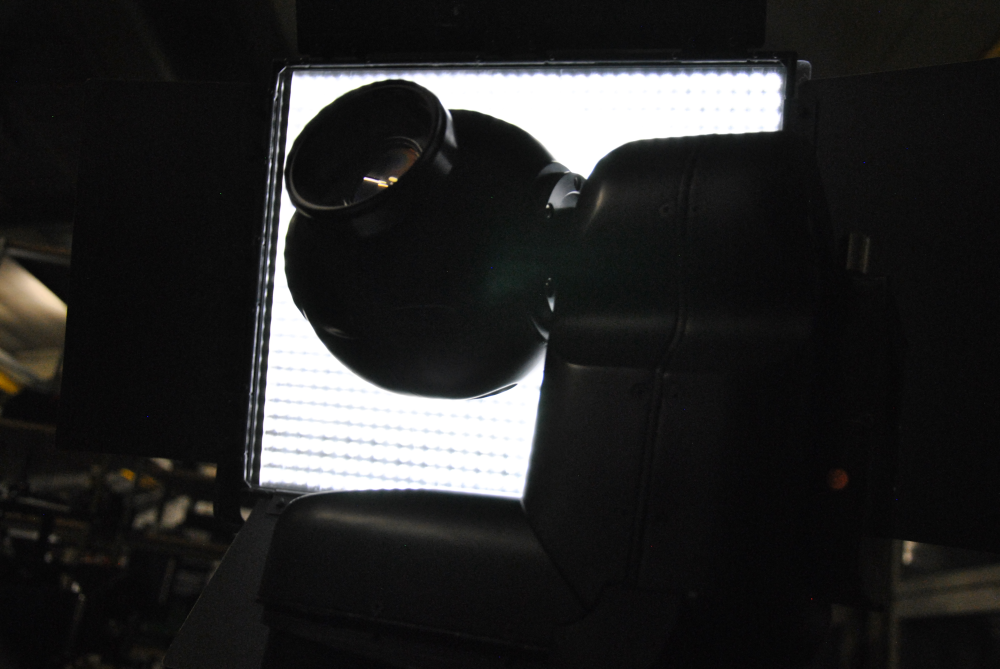
\includegraphics[height=50mm]{images/Titelblatt}\par
        \graphicscaption{Kamerakopf}
    \end{minipage}%
    \begin{minipage}[t][][t]{0.5\textwidth}
        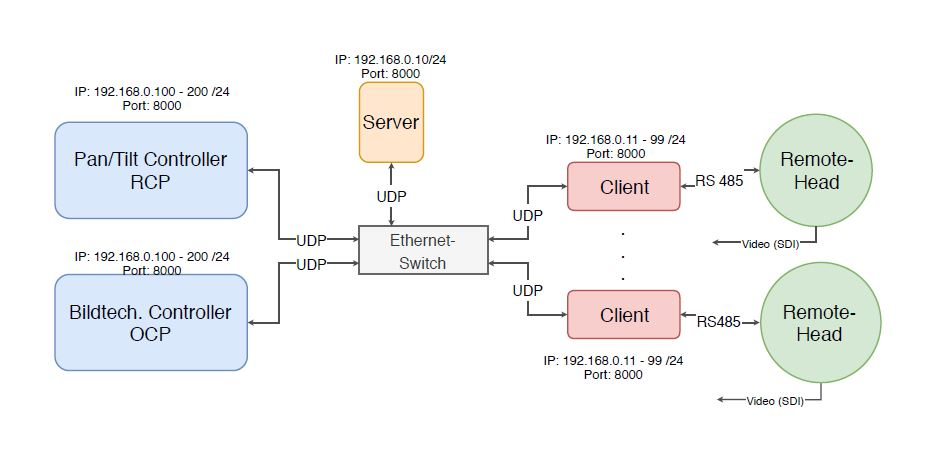
\includegraphics[height=40mm]{images/aufbau}\par
        \graphicscaption{Technischer Aufbau}
    \end{minipage}
}

\fscontent{
    \section{Bestehendes System}
    Das bestehende System wurde als eine spezielle Client-Server Struktur realisiert. Kommuniziert wird über UDP/Ethernet sowie RS485. Die Kameraköpfe sowie der Kontroller sind beim Server als Clients angemeldet. Dieser agiert nur als Vermittler, und leitet kommunikationspakete an die entsprechenden Clients weiter. Der Kontroller besitzt ein Touchdisplay als zentrales Bedienelement und einen 3-Achsen Joystick zur Kamerakopfsteuerung.

    \section{Systemanforderungen}
    Der neue Kontroller muss alle Funktionen des bestehenden beherrschen. Da das System in Echtzeit bedient wird, muss es Softrealtime-Anforderungen gerecht werden. Zusätzlich muss der Controller nebst der Remotekopfsteuerung, auch die Kamerasteuerung wie z.B. Blende und Weissabgleich bewältigen. Die Steuerungselemente dafür sollen optional als andockbares separates Bedientterminal am Kontroller angeschlossen werden können.

    \section{Gewählter Ansatz}
    Als Kernsystem soll ein embedded Linux dienen. Um die Machbarkeit aller Anforderungen aufzuzeigen wurde mit einem Raspberry Pi3+ gearbeitet. Dieses Board hat genügend Rechenleistung und verfügt über alle gängigen Schnittstellen wie Ethernet, I2C und SPI. Auf dem Touchdisplay läuft ein auf dem Qt Framework basierendes GUI. Es konnte erfolgreich mit dem bestehenden System über die vorgegebenen Protokollstruktur über UDP kommuniziert werden. Das System ist selbst ohne spezielle Kerneloptimierungen Soft-Realtime fähig.
}

\infobox{Eckwerte vom Prototypensystem}{%
    \begin{minipage}[t][][b]{0.45\textwidth}
        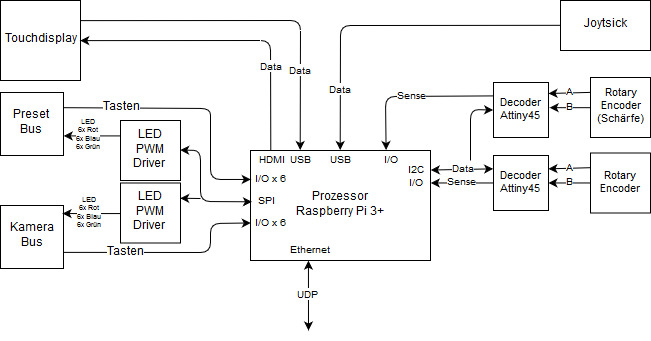
\includegraphics[width=\textwidth]{images/Blockschaltbild}
    \end{minipage}
    \hfill
    \begin{minipage}[t][][b]{0.55\textwidth}
    	\begin{itemize}
    		\item Architektur: Embedded Linux (Raspberry Pi3+, ARM Cortex-A53)
    		\item Reaktionszeit: System $25\mu s$, Toucheingaben $3ms$
    		\item Ethernetanbindung ans BBM Net
    		\item Custom Rotary Encoder SW \& HW (Attiny45) für möglichst ressourcenschonende Ansteuerung über I2C
    		\item 3-Achsen USB Joystick zur Kamerakopfsteuerung
    		\item 5 Zoll Kapazitives Touch Display mit state-of-the-art GUI (Qt)
    	\end{itemize}
    \end{minipage}
}
